\hypertarget{wrapper}{%
\subsection{Wrapper}\label{wrapper}}

\hypertarget{motivation}{%
\subsection{Motivation}\label{motivation}}

This pattern suggests to find at least one person to fill an important
role managing the project's public interface, and keeping participants
up to date about activities.

\hypertarget{context}{%
\subsection{Context}\label{context}}

You are part of an active, long-running, and possibly quite complex
project with more than a handful of participants. How do you manage?

\hypertarget{forces}{%
\subsection{Forces}\label{forces}}

\begin{quote}
\Sinterface\ \textbf{Interface}: the project shows people how they can use it.\\
\Sfamiliar\ \textbf{Familiarity}: the leader/follower dichotomy is easy to understand.\\
\Sequity\ \textbf{Equity}: peeragogy aims for fairness.
\end{quote}

\hypertarget{problem}{%
\subsection{Problem}\label{problem}}

In an active project, it can be effectively impossible to stay up to
date with all of the details. Not everyone will be able to attend every
meeting (see {{Heartbeat}}) or read every email. Project participants
can easily get lost and drift away. The experience can be much more
difficult for {{Newcomers}}: joining an existing project can feel like
trying to climb aboard a rapidly moving vehicle. Information overload is
not the only concern: there is also a problem with missing information.
If key skills are not shared, they can quickly become bottlenecks (see
{{Carrying capacity}}).

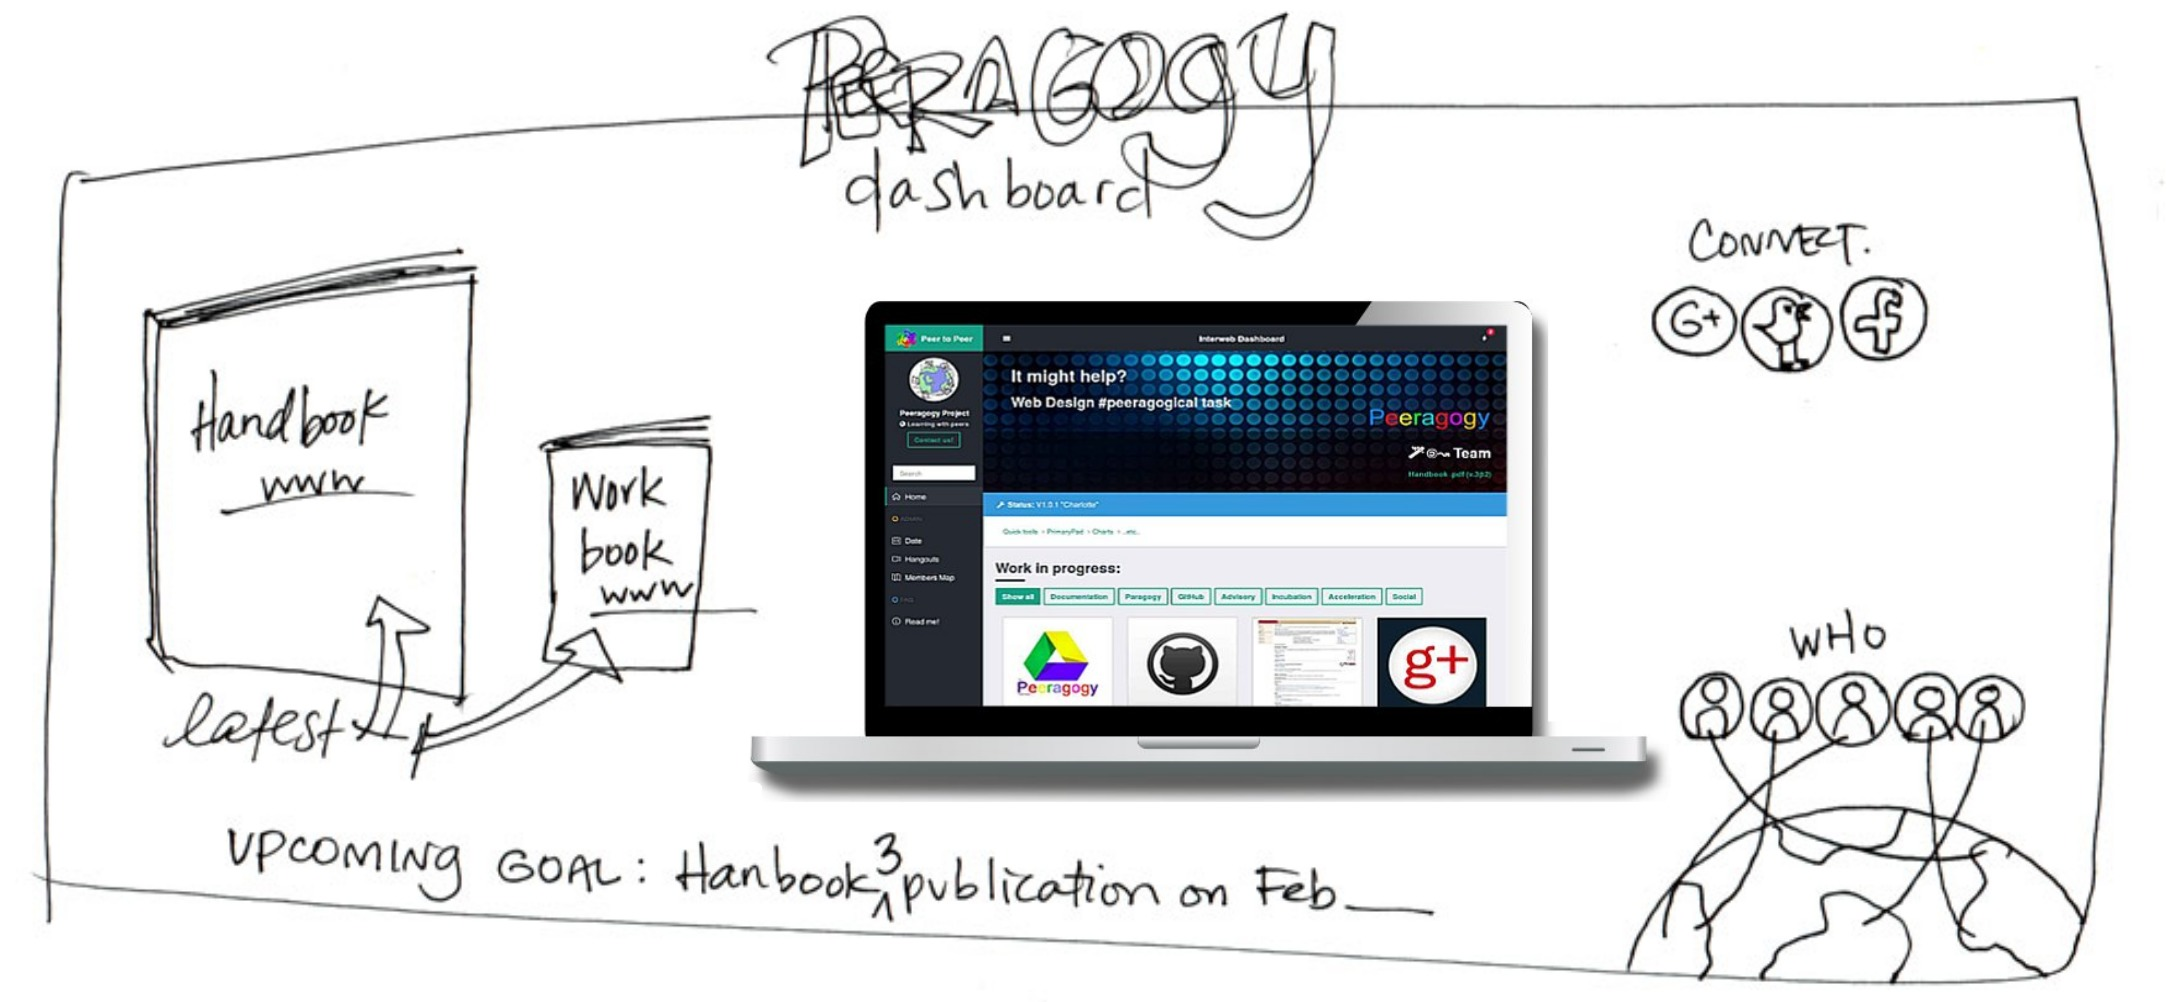
\includegraphics{images/dashboard_design.jpg} \emph{Design for a
Peeragogy project dashboard (sketch by Amanda Lyons, prototype by
Fabrizio Terzi).}

\hypertarget{solution}{%
\subsection{Solution}\label{solution}}

Someone involved with the project should regularly create a wrap-up
summary, distinct from other project communications, that makes current
activities comprehensible to people who may not have been following all
of the details. In addition, project members should keep other
informative resources like the landing page, {{Roadmap}}, and
documentation up to date. Check empirically to see if they really show
interested parties how they can get involved. Building on the idea of a
``project dashboard,'' we can guide potential contributors to live help;
we can then see what questions they ask.\footnote{\url{https://gitter.im/orgs/Peeragogy/rooms}}
{{Wrapper}} is both a role, and, sometimes, an artifact. Our
\emph{Handbook}'s cover literally wraps up its contents; the
collaboratively written chat notes from our weekly Hangouts give a
collaboratively-written overview of what was discussed in the meeting.
Meetings themselves can be structured to give people a chance to sum up
what they've accomplished during the week, as well as any problems they
are running into. Between meetings, each participant is advised to
maintain some sort of ``learning log'' in the form of a personal
{{Scrapbook}}, so that outstanding concerns are surfaced and available
to discuss.

\hypertarget{rationale}{%
\subsection{Rationale}\label{rationale}}

According to the theory proposed by Yochai Benkler, for free/open
``commons-based'' projects to work, it is important for participants to
be able to contribute small pieces, and for the project to have a way to
stitch those pieces together {{[}1{]}}. The {{Wrapper}} helps perform
this integrative stitching function. If you value participation, you may
have to do some serious work to facilitate access to process.

\hypertarget{resolution}{%
\subsection{Resolution}\label{resolution}}

Well-maintained records chronicle the project's history; up-to-date
documentation makes the project more robust; a coherent look-and-feel
offers an accessible \textbf{interface} to the outside world. Regularly
circulated summaries can help to engage or re-engage members of a
project, and can give an emotional boost to peeragogues who see their
contributions and concerns mentioned, giving less engaged participants
the \textbf{familiar} experience of ``following'' someone else's
updates. People will judge from experience whether the project strives
for \textbf{equity} or strives to maintain hidden power differentials.

\hypertarget{example-1}{%
\subsection{Example 1}\label{example-1}}

There are many data streams around the Wikimedia project. They comprise
an elaborate {{Wrapper}} function for the project, with components that
range from Today's Featured Article, which appears on the front page of
Wikipedia, to formal annual reports from the
nonprofit.\footnote{\url{https://en.wikipedia.org/wiki/Wikipedia:Today\%27s_featured_article}},\footnote{\url{https://wikimediafoundation.org/wiki/Annual_Report}}

\hypertarget{example-2}{%
\subsection{Example 2}\label{example-2}}

In-person meetings are just as relevant for contemporary humans as they
were a century ago, even though we have learned more about how to
assemble on the fly {{[}2{]}}. Getting together for conventions, dance
parties, and commencement ceremonies could comprise an important part of
the future university's {{Wrapper}} function, even if these events do
not always take place in one specific Assembly Hall.

\hypertarget{whats-next-in-the-peeragogy-project}{%
\subsection{What's Next in the Peeragogy
Project}\label{whats-next-in-the-peeragogy-project}}

Let's make sure we have protocols in place that enable us to share
progress, and to revise our ``next steps'' if people are getting stuck.
Let's improve the interaction design for peeragogy.org so that it's
clear how people can get involved.

\hypertarget{references}{%
\subsection{References}\label{references}}

\begin{enumerate}
\def\labelenumi{\arabic{enumi}.}
\item
  Y. Benkler. 2002. Coase's Penguin, or Linux and the Nature of the
  Firm. \emph{Yale Law Journal} 112: 369.
\item
  Howard Rheingold. 2007. \emph{Smart mobs: The next social revolution}.
  Basic books.
\end{enumerate}

\begin{center}\rule{0.5\linewidth}{0.5pt}\end{center}
